\section{Incrementando a Hydra com a Realidade Aumentada}
\label{sec:arHydra}

	Conforme visto, a Hydra auxilia no redirecionamento de recursos de um dispositivo para outros mais
	adequados no ambiente. Sua interação é feita de maneira sugerida, de forma que são exibidos para a
	seleção do usuário apenas aqueles que lhe são compatíveis. Nesta abordagem, cabe ao usuário
	realizar a ligação entre o nome do dispositivo exibido nas opções e o recurso que deseja utilizar.	
	No entanto, o usuário pode ter dificuldades de associar o nome exibido e ao dispositivo contendo o
	recurso desejado.
	
	A figura \ref{fig:sala_computadores} mostra uma sala com computadores com características físicas
	semelhantes, numerados de 1 à 12. Considere que um usuário esteja utilizando o computador de
	número 4 e deseje utilizar um recurso específico de um outro computador (assuma que todos os
	computadores estejam disponibilizando seus recursos no ambiente). A Hydra mostrará uma lista de
	recursos passíveis de redirecionamento e ficará aguardando a seleção de um dispositivo. Suponha que o
	recurso desejado esteja disponível no computador de número 10 e o usuário o selecione. Nesse
	momento, o usuário terá que identificar qual computador foi selecionado na lista fornecida pela
	Hydra. No entanto, como há uma grande similaridade nas características físicas, o usuário terá
	dificuldades de associar o nome exibido, pela lista da Hydra, ao equipamento selecionado.
	
	\begin{figure}[htb]
		\centering 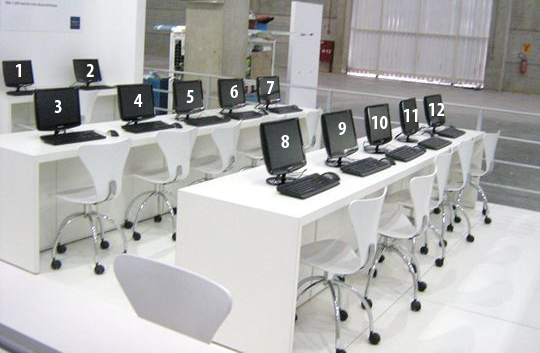
\includegraphics[scale=0.65]{figuras/cap3/sala_computadores.png}
		\caption{\textit{Sala com computadores.}}
		\label{fig:sala_computadores} 
	\end{figure}


    A ARHydra (\textit{Augmented Reality Hydra}) visa amenizar esta tarefa fazendo uso de técnicas de
    Realidade Aumentada. A inserção de informações através de objetos virtuais facilitará na
    identificação dos dispositivos no ambiente inteligente. Os dispositivos serão mapeados através de
    marcadores estrategicamente localizados no dispositivo. De modo que, novas informações a
    respeito dos recursos disponibilizados pelo dispositivo fossem apresentadas para o usuário no
    momento de sua localização.
    
    Esse novo meio de visualização dos recursos proverá uma nova forma de interação entre o
    usuário e o ambiente inteligente. Desta forma, a utilização das facilidades de redirecionamento
    de recursos provida pela Hydra pode ser incrementada com uma visualização, e localização,
    simplificada destes.
    
\subsection{Marcadores na ARHydra}

	Aplicações para a realidade aumentada utilizam marcadores com características próprias, como é
	o caso das aplicações ARToolkit e ARTag. A maior parte dos trabalhos que utilizam esses
	marcadores, associam o código de identificação extraído do marcador a um objeto virtual
	pré-definido. Essa relação causa uma dependência de um mapeamento prévio de todos os objetos 
	virtuais e seus respectivos códigos de identificação, proporcionando uma limitação na interatividade 
	entre novos marcadores.
	
	A ARHydra segue uma estratégia diferente. Utiliza características que favoreçam o reconhecimento e
	a extração de informações através de seus marcadores, sem a necessidade de uma tabela de
	mapeamento. Esse comportamento híbrido proporciona uma interatividade na identificação dos
	marcadores, uma vez que a disponibilidade dos recursos dependem dos dispositivos presentes no
	ambiente.
	 
	A escolha do código QRCode, para identificação dos marcadores, baseia-se na possibilidade de
	inserção de caracteres alfanuméricos, na rápida leitura e na tolerância a erros oferecidas por
	esse código bidimensional. Possibilitando assim, uma forma simplificada para a extração da
	identificação dos dispositivos no ambiente inteligente. 
	
	A figura \ref{fig:arhydra_marcador} exemplifica o marcador utilizado pela ARHydra. Na primeira
	parte da figura é apresentado um marcador utilizado pela aplicação ARToolkit. Em seguida, um
	código QRCode responsável por armazenar alguma informação relevante a respeito do dispositivo. A
	junção dos mesmos formará um marcador constituído de bordas pretas, aos quais delimitam o marcador
	e favorecem uma forma rápida de localização, e o QRCode no centro do marcador, responsável pela
	identificação do marcador.
	
	\begin{figure}[h]
		\centering \includegraphics[scale=0.5]{figuras/cap3/marcador_arHydra.png}
		\caption{\textit{Marcador utilizado na ARHydra.}}
		\label{fig:arhydra_marcador} 
	\end{figure}
	
\subsection{Interação no ambiente}

	Considere o seguinte exemplo de interação da ARHydra com o ambiente. Suponha um 
	\textit{smart space} composto por:
	
	\begin{enumerate}
	  \item Macbook: disponibiliza os recursos de \textit{webcam}, saída de vídeo, \textit{mouse} e
	  teclado;
	  \item \textit{Smartphone} Galaxy SII: disponibiliza os recursos de câmera, mouse e teclado;
	  \item iMac: disponibiliza os recursos de saída de vídeo, \textit{mouse} e teclado.
	\end{enumerate}
	
	No macbook terá uma aplicação utilizando o \textit{uOS} disponibilizando seus recursos através de
	\textit{UpDriver's}, sendo este dispositivo mapeado no ambiente através de um marcador reconhecido
	pela ARHydra. O \textit{smartphone} ficará responsável pela execução da aplicação ARHydra. Por
	fim, a aplicação Hydra será executada no iMac. 
	
	O uso dos marcadores, alinhado com a mobilidade com que o \textit{smartphone} pode interagir com o
	ambiente, faz com que a aplicação ARHydra seja utilizada no \textit{smartphone} do usuário. Essa
	interação possibilita ao usuário uma melhor forma de localização e seleção do recurso disponível.
	
	A figura \ref{fig:apresentacao_arhydra} exemplifica o uso de um marcador para identificar o dispositivo no
	ambiente. Como etapa inicial ilustrada através da figura \ref{fig:visualizacao_qrcode}, há uma
	busca por esse marcador inserido no ambiente, ao qual posteriormente será feito uma tentativa de
	reconhecimento para obtenção da informação contendo os recursos disponibilizados. Com a conclusão
	bem sucedida da etapa anterior, o os recursos serão apresentados ao usuário, conforme ilustrado na
	figura \ref{fig:visualizacao_obj}. Essa exibição é feita utilizando técnicas da realidade
	aumentada. Por fim, a aplicação ARHydra possibilita ao usuário escolher qual recurso deseja que
	seja redirecionado para a Hydra.
	
	\begin{figure}[htb]
		\centering
			\subfloat[Visualização do marcador]{
				\label{fig:visualizacao_qrcode}
				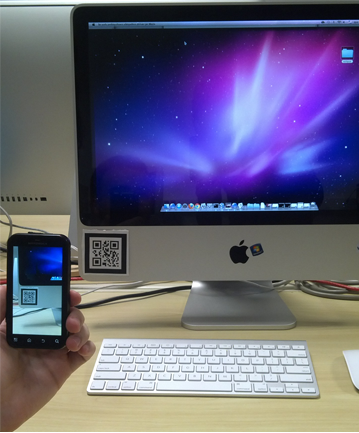
\includegraphics[width=0.45\textwidth]{figuras/cap3/visao_mac.png}
			}
			\subfloat[Visualização do objeto virtual]{
				\label{fig:visualizacao_obj}
				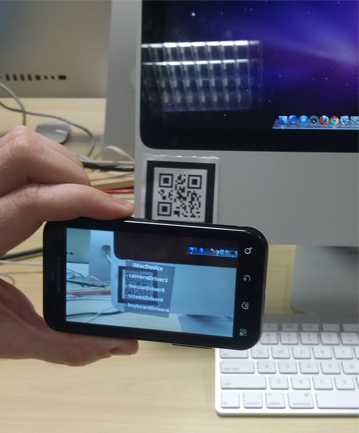
\includegraphics[width=0.45\textwidth]{figuras/cap3/visao_qrcode.png}
			}
		
		\caption{\textit{(a) Exemplo da visão do usuário para a busca do marcador do dispositivo. (b)
		Exemplo da visualização do objeto virtual apresentando os recursos disponíveis}}
		\label{fig:apresentacao_arhydra} 
	\end{figure}
	
	
	A interação da ARHydra no ambiente inteligente segue os passos observados na figura~\ref{fig:arhydra_interacao}:

	\begin{figure}[h] 
		\centering 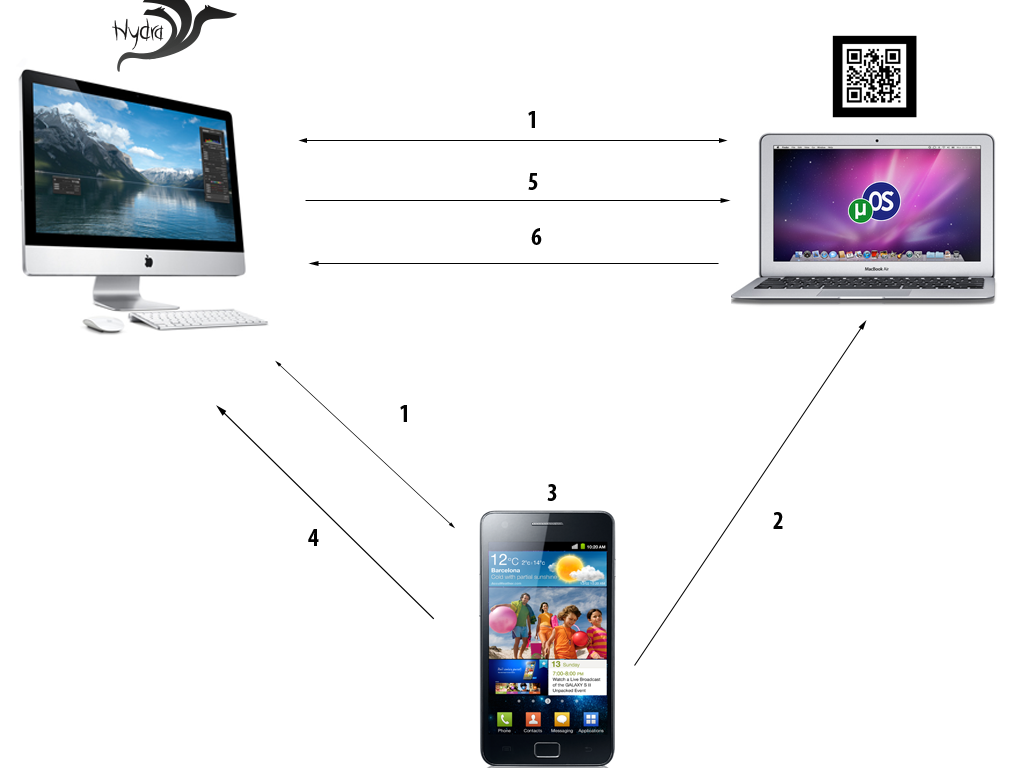
\includegraphics[scale=0.45]{figuras/cap3/integracao_arhydra.png}
		\caption{\textit{Integração Hydra com o ambiente.}}
		\label{fig:arhydra_interacao} 
	\end{figure}
	
	\begin{enumerate}
	  \item A Hydra implementa o mecanismo de descoberta de novos dispositivos e os registra os
	  dispositivos encontrados em sua base de dados;
	  
	  \item A ARHydra procura o marcador identificador do Macbook;
	  
	  \item Faz a reconhecimento e decodificação do marcador encontrado, busca os recursos disponíveis
	  do dispositivo e apresenta esses recursos na tela do \textit{smartphone} com os recursos
	  providos pela realidade aumentada, possibilitando ao usuário selecionar um recurso disponível.
	  
	  \item Caso o usuário selecione um recurso, a ARHydra faz uma requisição à Hydra para que
	  redirecione o recurso selecionado do Macbook para o uso na Hydra.
	  
	  \item A Hydra recebe a solicitação vinda do \textit{smartphone}, solicita o registro do
	  recurso selecionado para a aplicação do \textit{uOS} executada no Macbook.
	  
	  \item A partir desse momento, o recurso do Macbook selecionado pela ARHydra será redirecionado
	  para o iMac.
	\end{enumerate}

	Com isso, a aplicação ARHydra complementa a interação do usuário com a Hydra, auxiliando na
	identificação visual dos dispositivos e no redirecionamento dos recursos disponíveis. 
 	

	
